\chapter{Wykład 15. Zarządzanie kontraktami w projekcie informatycznym}

\section{Formy wynajmu prac}
% strona 13

Z powodu niewielkich rozmiarów naszej firmy, a także braku specjalistów z niektórych dziedzin postanowiliśmy zlecić część zadań innym firmom. Dwa główne zadanie z którymi związane będzie zlecenie prac to opracowanie i stworzenie szaty graficznej dla naszego produktu, a także zapewnienie oraz utrzymanie serwerów na potrzeby naszego przedsiębiorstwa. Dla naszej firmy proponujemy następujące formy wynajmu prac:
\begin{itemize}
\item Najlepsze osiągalne rozwiązania (best-of-breed) – w każdym obszarze planujemy rozważyć zlecenie zadań związanych z nim na zewnątrz, albo pozostawienie ich wewnątrz firmy. Kupowanie rozwiązań dla różnych obszarów od różnych firm pozwoli nam zapewnić najlepsze dla przedsiębiorstwa rozwiązanie.
\item Partnerstwo – zawarcie umowy z inną firmą zajmującą się szeroko pojętą grafiką, pozwoli nam zapewnić szatę graficzną naszego produktu na wysokim poziomie, a także przetransferować ryzyko związane z brakiem grafików w naszym zespole.
\item Outsourcing – planujemy oddelegować do zewnętrznej firmy zadań związanych z dostarczeniem i utrzymaniem serwera na potrzeby naszego przedsiębiorstwa.
\end{itemize}

% ===========================================================================


\section{Szkic kontraktu}
% strona 31

\begin{figure}[!h]
\centering
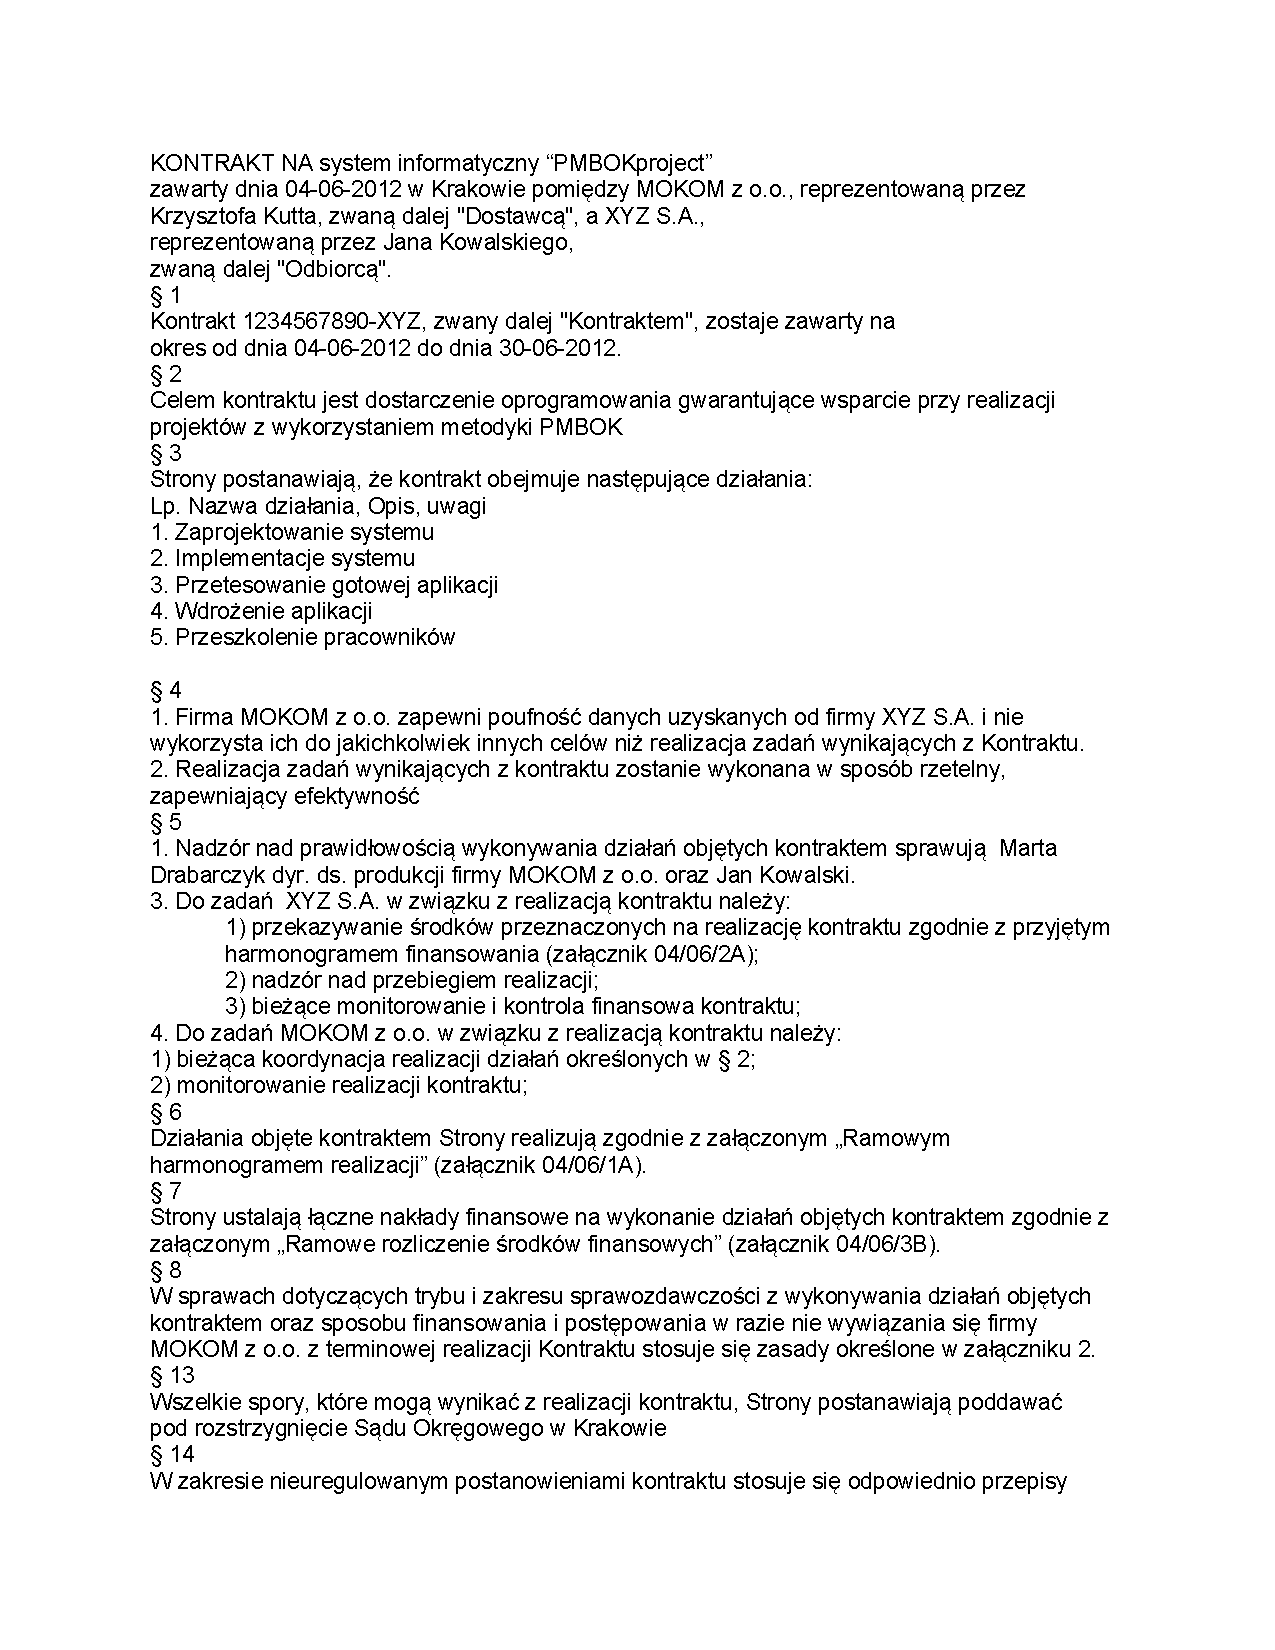
\includegraphics[width=1.1\textwidth]{szkicKontraktu.pdf}
\caption{Szkic kontraktu}
\label{fig:szkicKontraktu}
\end{figure}

% ===========================================================================

\section{Wybór prac, które należy zlecić. Wybór dostawcy}
% strona 50

Ten wirtualny warsztat jest beznadziejny.

% ===========================================================================

\section{Wybór kontraktu dla organizacji oraz podwykonawców}
% strona 50

Ten wirtualny warsztat jest beznadziejny.
